\chapter{Indledning}
Vi har i dette projekt arbejdet med design og udvikling af et blodtryks målesystem. Ideen bag vores system blev udtænkt og udarbejdet med viden om en blodtryksmåler på en operationsstue på Herning Sygehus. Vores opstillede krav samt design til systemet, blev derfor lavet ud fra de oplysninger vi fik af en sygeplejerske\footnote{Anæstesi sygeplejerske Charlotte Høj, Herning Sygehus} på Herning Sygehus. Vi ønskede altså at lave et blodtryksmålersystem, som er så virkelighedsnært som muligt. Det design og de funktionaliteter vi efterstræbte at få opfyldt i vores projekt var derfor EKG, systoliske samt diastoliske blodtryk og iltmætning i blodet. Dette ønskede vi at få implementeret og hermed få grafer og værdier vist på en brugergrænseflade, som lever op til de standarder der ses på operationsstuer i dag. \\
\\
Baggrunden for dette projekt er, at man i klinisk praksis har behov for kontinuert at observerer patientens blodtryk. Det er i særdeleshed på intensiv afdelinger og operationsstuer, at man ønsker at lave invasiv blodtryksmåling. Ved invasiv blodtryksmåling kan man monitorere patientens fysiske tilstand under eksempelvis operation. Blodtrykket kan give en identifikation af blødning, smerter og hvor dybt patienten sover under narkosen. Denne overvågning giver det sundhedsfaglige personale en ekstra tryghed og sikkerhed om patientens tilstand under operation. \\
\\
Denne projekt rapport vil give en kort beskrivelse af vores samlede system samt krav hertil. Der vil være en udspecificeret projektbeskrivelse, som vil give et indblik i vores vej frem til det endelige resultat, og som også vil beskrive både de til- og fravalg vi har måttet tage, for at nå frem til netop det system vi ønskede at realiserer og præsenterer. Der har i den forbindelse været nogle ideer og ønsker, som ikke har været realistiske og tidsmæssigt mulige at opfylde og vil derfor være beskrevet i fremtidigt arbejde. Slutteligt vil derfor være en samlet konklusion på projektarbejdet.
\chapter{Projektformulering og afgrænsning}
\section{Oversigt over projektdeltagere og hovedansvarsområder}
Vi har i dette projekt valgt at dele projektets deltagerer op i to grupper med hver deres hovedansvarsområder. En som har beskæftiget sig med hardware og en som har beskæftiget sig med software. Derudover valgte vi i starten af forløbet at udvælge en projektleder, hvis opgaver bestod i at lave dagsorden for hvert møde, sørge for at deadlines blev overholdt, træffe endelige beslutninger og holde et overordnet overblik over projektet. Vi valgte også en procesleder hvis opgaver bestod i opgavestyring, godt arbejdsmiljø i gruppen og planlægning af projektforløbet. \\
\\
Under projektforløbet valgte vi at ændre denne rollefordeling, idet den generelle arbejdsfordeling samt arbejdsindsats i gruppen ikke fungerede optimalt. Vi valgte, at kun et gruppemedlem skulle varetage rollen som projektleder og procesleder, men at opgaver herunder kunne uddelegeres hvis nødvendigt. Denne leder blev i fællesskab valgt og baggrunden for dette valg var, at vi ønskede en leder som både havde viden og indflydelse på hardware og software, samt kunne træde i kræft hvis gruppearbejdet og deltagernes indsat ikke opfyldte den forventningsafstemning, som står skrevet i vores samarbejdskontrakt. \\\\
\begin{tabular}{| l | l |} \hline
\textbf{Hardware} & \textbf{Software}\\\hline
Brian Hansen & Ida Mark Skovbjerg \\\hline 
Mohamed Hussein Mohamed & Mette Østergård Knudsen \\\hline
Khaled Edwan & Line Skov Larsen  \\\hline 
\end{tabular}
\\
\begin{tabular}{| l | l |} \hline
\textbf{Fulde navn} & \textbf{Initialer}\\\hline
Ida Mark Skovbjerg & IMS \\\hline 
Line Skov Larsen & LL \\\hline
Mette Østergård Knudsen & MK  \\\hline 
Brian Hansen & BH \\\hline
Mohamed Hussein Mohamed & MM \\\hline 
Khaled Edwan & KE \\\hline
\end{tabular}



Hvad vil vi
Hvad skal produktet kunne
Løsning
Fremtiden
Deltager; Fulde navn og initialer


\chapter{Hjertet}
Hjertet er en muskel, der fungere som en pumpe i kroppen. Hjertet pumper det iltede blod ud til resten af kroppen gennem arterie- og vene systemer. Når blodet passere ud af hjertet igennem arterierne sker der et tryk mod arterievæggene, dette kaldes blodtrykket. Man benytter blodtrykket til at bedømme kraften og mængden af det blod, som pumpes ud af hjertet. Blodtrykket inddeles i to typer, systolisk og diastolisk. \\\\
Systolen angives som den kraft, der skabes når der kommer pres på karvæggen i arterierne. Dette sker i hjertets sammentrækningsfase, hvor blodet pumpes ud i arterierne. Systolen i et normalt blodtryk i hvile vil ligge i intervallet 100-140mm Hg og ved forhøjet blodtryk er værdien for trykket over 140 mm Hg. Diastolen angiver hjertets hvilefase og ses mellem to sammentrækninger. I denne fase fyldes ventriklerne med blod. Den normale værdi for diastolen ligger i intervallet 60-90 mm Hg. Hvis den overstiger 90 mm Hg anses blodtrykket for at være forhøjet. Udover systolen og diastolen kan også middeltrykket angives. Denne udregnes ved formlen: $middeltryk = \dfrac{2}{3}\cdot diastolisk + \dfrac{1}{3}\cdot systolisk$. \cite{blodtrykwiki}
\\\\
Hypertension defineres som forhøjet systole, forhøjet diastole eller både forhøjet systole og diastole. Hypertension belaster hjertet, og medføre en øget risiko for udviklingen af apopleksi. Det er også forbundet med flere medicinske tilstande såsom arteriosklerose, hjerteinsufficiens og nyreskader.\cite{hypertension}
\\\\
Ser man på anatomien bag blodtrykket og blodtryksændring, består dette af kredsløbssystemet, som omfatter blodets kredsløb, hjertet og lymfesystemet. Blodkredsløbet er et langt netværk af arterier og vener, som har til opgave at føre iltet blod ud til hver celle i kroppen, samt opfange affaldsprodukter fra celler og væv.\cite{pulmonal} I lungekredsløbet udskilles affaldsprodukter og blodet iltes. Det er hjertet der pumper blodet ud i dette netværk, så blodet hele tiden er i bevægelse. Arterierne transportere blodet væk fra hjertet, og venernes opgave er at transportere blodet mod hjertet. \\\\
Kredsløbet kan funktionelt og anatomisk inddeles i to dele: Det pulmonale kredsløb og det systemiske kredsløb.De to kredsløb fungerer i symbiose mellem hjertets højre hjerte kamre og hjertets venstre hjertekamre. Højre siden pumper blodet gennem det pulmonale kredsløb, og venstre side pumper blodet rundt i det systemiske kredsløb. Hver pumpe består af to kamre: et forkammer, atrium og et hovedkammer, ventriklen. Det pulmonale kredsløbs primære funktion er at levere blodet til lungekredsløbet hvor blodet iltes. Hjertets højre side modtager iltfattigt blod og CO2-rigt blod via v. Cava superior og inferior fra det systemiske kredsløb og pumper det videre ind i lungekredsløbet gennem det pulmonale kredsløb via pulmonal aterierne. Fra lungerne løber det nu iltrige og CO2-fattige blod tilbage til venstre side af hjertet, som derfra pumper det videre til det systemiske kredsløb via aorta.\cite{pulmonal}
\begin{figure}[H]
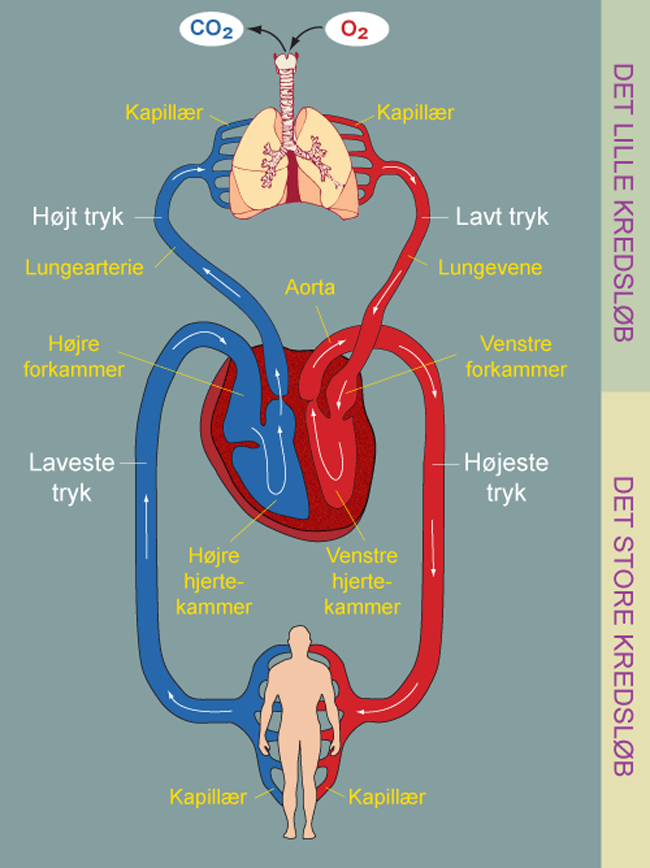
\includegraphics[width =0.5\textwidth , center]{billeder/hjertet}
\caption{\textbf{Det lille og det store kredsløb. Motoren der driver det hele er hjertet.\cite{hjertet}}}
\end{figure}


\chapter{Systembeskrivelse}



\chapter{Krav}
Hvilke krav der stilles til produktet udarbejdes i en kravspecifikation. Denne kravspecifikation består af en række Use cases. Disse Use cases beskriver interaktionen mellem aktørerne og systemet. Use casene har til formål at specificere, hvilke krav der stilles til produktet. Kravene opstilles ud fra hvad kunden ønsker samt hvad leverandøren finder muligt at realisere. \\ \\
Der er nogle obligatoriske krav til produktet, der skal opfyldes. Disse krav er bl.a at systemet skal kunne kalibrere blodtrykssignalet og foretage en nulpunkts justering. Desuden skal blodtrykssignalet vises kontinuerligt, hvilket betyder, at signalet skal vises grafisk samtidigt med at det bliver hentet/indsendt fra hardwaren. Disse målte data skal efter de er blevet behandlet gemmes i en database.\\
Et af de obligatoriske krav er desuden at der skal være et digitalt filter der kan tilgås når programmet kører. Dette filter skal både kunne slås til og fra. Dette filter skal sørge for at signalet haves i to forskellige modes; et diagnose mode, hvor signalet er råt med alle udsving, og et monitor mode, hvor signalet er filtreret og afrundet.\\\\
Foruden disse obligatoriske krav er det valgt, at det skal være muligt starte og stoppe målingen. Når målingen er startet skal det være muligt at kunne justere grænseværdierne for systolen og diastolen, så disse værdier kan tilpasses. Når signalets værdier så kommer over grænseværdien, skal en alarmering begynde. Denne alarm skal kunne udsættes i et minut, dog kun alarmens lyd, så værdien blinker fortsat, så det stadig er tydeligt hvilken grænseværdi der er overskredet.\\
Systemet består af en computer med en programkode, en NI-DAQ, et lavpas filter, en forstærker, en transducer og en væskesøjle.
Systemet gør det muligt at få arterietrykket sendt ind i systemet igennem hardwaren. Arterietrykket dannes i denne prototype af en væskesøjle, som levere et tryk til en transducer, herefter sender transduceren signalet videre til hardwaren, hvor et lavpasfilter, filtrerer signalet, hvorefter en forstærker forstærker signalet. Dette signal sendes derefter igennem NI-DAQ ind i systemet, som derefter behandler og analyserer signalet.\\
Den fulde beskrivelse af de udarbejdede Use cases (fully dressed Use case skema) findes i dokumentationen.
\begin{figure}[H]
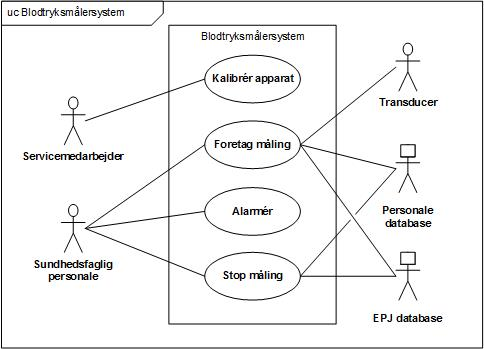
\includegraphics[width =0.7\textwidth , center]{billeder/UseCaseDiagram}
\caption{Use Case diagram. Dette diagram viser aktørernes interaktion med systemet.}
\end{figure}
\section{Aktørbeskrivelse}
Ud fra use case diagrammet ses de seks aktører; \textit{Sundhedsfaglig personale}, \textit{Transducer}, \textit{EKG patient}, \textit{EPJ database}, \textit{Personale database} og \textit{Servicemedarbejder}. Det er disse aktører der interagerer med systemet.
\subsection{Sundhedsfaglig personale}
Det er det sundhedsfaglige personale der er den aktør der påsætter måleudstyret på patienten. I dette tilfælde vil patienten være en transducer, hvilken er tilsluttet en væskesøjle. Det sundhedsfaglige personale er desuden den aktør der interagere med systemet; logger på og foretager en måling. Det sundhedsfaglige personale har dermed tilgang til de viste målinger på brugergrænsefladerne; startskærm og hovedskærm
\subsection{Transducer}
Transduceren er i projektet den aktør der agere som patienten, denne består af en væskesøjle der er påsat en tryktransducer. Væskesøjlen levere et tryk i mmHg videre til tryktransduceren, og dette signal, der virker som arterietrykket, sendes videre i hardwaren, som behandler signalet. Derfor er denne aktør kilden til måleresultaterne for systole, diastole og middeltryk. 
\subsection{EKG-patient}
EKG patienten er den aktør som er kilden til EKG-kurven, idet vi ikke har en rigtig patient, hvorfra både EKG og blodtryk kan fås fra. Idet det er fra denne aktør at EKG-kurven findes er det fra denne aktør, pulsen kan bestemmes.\\
Værdierne for denne aktør hentes fra PhysioBank ATM.
\subsection{Servicemedarbejder}
Denne aktør, Servicemedarbejder, er den aktør, der står for at foretage kalibreringen. Dette gør Servicemedarbejderen ved at påsætte systemet til kalibrerings systemet, og indtaster de værdier for tryk (mmHg) og spænding (Volt), som måles ved tre forskellige målepunkter på en væskesøjle, hvorefter en kalibreringsværdi findes af systemet.
\subsection{EPJ database}
EPJ databasen, er databasen, hvori patientdata ligger samt den database hvori grafer og måleresultaterne, der bestemmes ved analysen, bliver gemt. Måleresultaterne er systole, diastole, middeltryk og pulsen.
Graferne for EKG-signalet og arteriekurven gemmes som tallister. Denne EPJ database skal simulere den database der fungerer på sygehusene i virkeligheden. Denne database kobler patienterne i denne database sammen med en sundhedsfaglig fra Personale databasen.
\subsection{Personale database}
Det sundhedsfaglige personales login informationer ligger i Personale databasen. Det er derfor denne database der indeholder informationer om det Sundhedsfaglige personale og dermed de informationer der benyttes til at tilgå systemet.
\section{Use case beskrivelse}
Use case diagrammet viser ligeledes de 4 Use cases der er for systemet: Kalibrér apparat, Foretag måling, Alamér og Stop måling. Disse Use cases er en beskrivelse af hvad systmet skal kunne og dermed beskriver de interaktioner der sker mellem aktørerne og systemet.
\\
\subsection{Use case 1: Kalibrér apparat}
Servicemedarbejderen skal i denne Use case foretage en kalibrering. Dette gøres ved at der er tre målepunkter på en væskesøjle, hvor en af disse vælges. På disse punkter måles spændingen (volt) og trykket (mmHg) aflæses fra væskesøjlen. Disse indtastes af Servicemedarbejderen ind i systemet igennem brugergrænsefladen; startskærmen. Herefter beregner systemet en kalibrerings værdi. Denne værdi bruges til at omskrive de indlæste værdier til en blodtrykskurve i mmHg.
\subsection{Use case 2: Foretag måling}
Denne Use case styrer målingerne af graferne der indhentes. For at dette kan gøres skal det Sundhedsfaglige personale først logge på systemet. Dette gør denne aktør ved at indtaste sit brugernavn og sin adgangskode på brugergrænsefladen; startskærmen. Når den sundhedsfaglige på logget på henter systemet de tilknyttede patienter, hvorefter det Sundhedsfaglige personale kan vælge den ønskede patient. Når Patienten er blevet valgt startes hovedskærmen, hvilken repræsenterer en blodtryksmålers brugergrænseflade. Her kan den Sundhedsfaglige starte målingen. Når dette gøres henter systemet arteriekurven og EKG-signalet. Dette bruges derefter af systemet til at beregne hhv. systole, diastole, middeltryk og puls. Systemet viser graferne kontinuerligt på hver sin graf og systole, diastole, middeltryk og puls vises som talværdier. Samtidig gemmer systemet automatisk kontinuerligt disse data i EPJ databasen. \\
Det vil være muligt for det Sundhedsfaglige personale at slå det digitale filter fra og til. Filteret er fra start slået til.\\
DEt er også muligt for det Sundhedsfaglige personale at justere grænseværdierne for systolen og diastolen, dette gøres for at indstille grænseværdierne mere individuelt for hver patient.\\
For at sikre at graferne der er hentet ligger rigtigt på graferne, kan det Sundhedsfaglige personale nulpunkts justere systemet, sådan at graferne kommer til at ligge rigtigt på akserne.
\subsection{Use case 3: Alarmér}
Alarmen startes af systemet, når en af grænseværdierne overskrides. Dette gør at grænseværdien der er overskredet blinker og at der starter en alarm lyd. Når alarmen kan endnu en grænse værdi overskrides, hvis dette sker begynder denne grænseværdi ligeledes at blinke, men der sker ikke noget med alarmlyden, denne fortsætter fra tidligere. \\
Det vil her være muligt for det Sundhedsfaglige af udsætte alarmen. Dette gøres ved at trykke på knappen, hvorefter at systemet stopper alarmens lyd i et minut, efter dette minut starter alarmens lyd igen. Grænseværdien/grænseværdierne der er overskredet fortsætter med at blinke indtil forholdene er normaliseret, altså indtil grænseværdien ikke længere er overskredet.
\subsection{Use case 4: Stop måling}
Det Sundhedsfaglige personale skal også stoppe målingen. Dette gøres ved at det Sundhedsfaglige personale interagere med hovedskærmen. Herefter vil det være muligt for det Sundhedsfaglige personale at logge 
\section{Ikke-funktionelle krav beskrivelse}
Ikke funktionelle krav er opsat efter FURPS+ metoden. Kravene er herefter blevet prioriteret efter MoSCoW.
\subsection{FURPS+}
\textbf{Functionality}\\
Funktionalitet er det brugeren ønsker sig. Dette omfatter også sikkerhedsrelaterede behov. Dette er krav til hvad programmet skal kunne af funktionalitet, f.eks. at programmet skal have et digitalt filter.\\\\
\textbf{Usability}\\
Hvor effektiv er produktet, set fra forbrugerens side, dette er det aspekt brugervenlighed ser på. Er produktet nemt at bruge. Hvordan bruges produktet; er der nogen brugergrænseflader. Det er herunder kravene til hvilke knapper der skal være på brugergrænsefladerne, og dermed også hvilke brugergrænseflader der skal være.\\\\
\textbf{Reliability}\\
Pålidelighed tager sig af aspekter som, hvor længe er det maksimalt at systemet må være nede. Er der fejl der kan forudses. Hvor præcist kan resultaterne vises. Er produktet let at vedligeholde; kan delene i produktet skiftes let.\\\\
\textbf{Performance}\\
Præstationen for produktet, handler om hvor hurtigt produktet er om at starte op og hvor hurtigt svartiden er. Hvor stor må svartiden maksimalt være. Så det er altså herunder, at det er beskrevet, hvor lang tid der går fra der er trykket på en knap, til at systemet svarer. \\\\
\textbf{S}uportability\\
Produktets support fortæller, om det er muligt at teste på produktet, om det er muligt at udvide produktet, installere og konfigurere produktet. Desuden om produktet er kompatibelt. Det er herunder programmets opbygnings model beskrives\\\\
\textbf{+}\\
Kunden kan have nogle yderligere behov, disse yderligere behov beskrives under +. Hvilke begrænsninger er der ved designet. Er der nogle krav for brugergrænsefladerne. Er der nogle fysiske eller implementerings krav. Er der dele der kan genbruges, herunder hele systemer eller dele af dem. Det er bl.a herunder at kravene til computeren der benyttes beskrives.\\
\url{http://agileinaflash.blogspot.dk/2009/04/furps.html}

\subsection{MoSCoW}
\textbf{Must}\\
De krav der bliver markeret som et must er de krav som produktet skal have. Altså det produktet skal have/indeholde.\\\\
\textbf{Should}\\
De krav der markeres som et should krav, er de krav til produktet der burde være med. Altså er det hvad produktet bør indeholde\\\\
\textbf{Could}\\
Kravene kan også markeres som could. Disse krav er de krav der kunne være gode at have med, men som ikke bliver prioriteret. Så det er kun, hvis man kan nu at få det med, at de skal være der.\\\\
\textbf{Would/Won't}\\
Det er ikke alle krav der skrives, der skal være gældende for produktet, disse krav markeres som would/won't. Det er altså disse krav som man ikke tager med eller de krav som ville være sjove at have med, men ikke har en betydning for produktet, men er en tilføjelse eller udvidelse. Det er disse krav der danner rammen for fremtidigt og videregående arbejde med projektet.
\chapter{Projektbeskrivelse}
\section{Projektgennemførelse}
Modellerne
\subsection{ASE-modellen}
Til udviklingen af dette produkt er der primært benyttet ASE-modellen. Modellen ses herunder. ASE-modellen er en udviklingsmodel, der er udarbejdet af Aarhus Ingeniørhøjskole. Denne model er en mellemvægtig semi-iterativ udviklingsproces, hvilken drives ud fra Use cases. Projektudviklerne fastlægger først en projektformulering, hvorfra en kravspecifikation kan udarbejdes, hvilke indeholder kravene fra kunden. Systemarkitekturen fastlægges ud fra kravspecifikationen, for derefter at designe og implementere de enkelte hardware og software dele hver for sig i iterationer. Til sidst fører dette til en accepttest, hvilken gennemføres, så der opstår een enighed mellem projektudviklerne og kunden.
\begin{figure}[H]
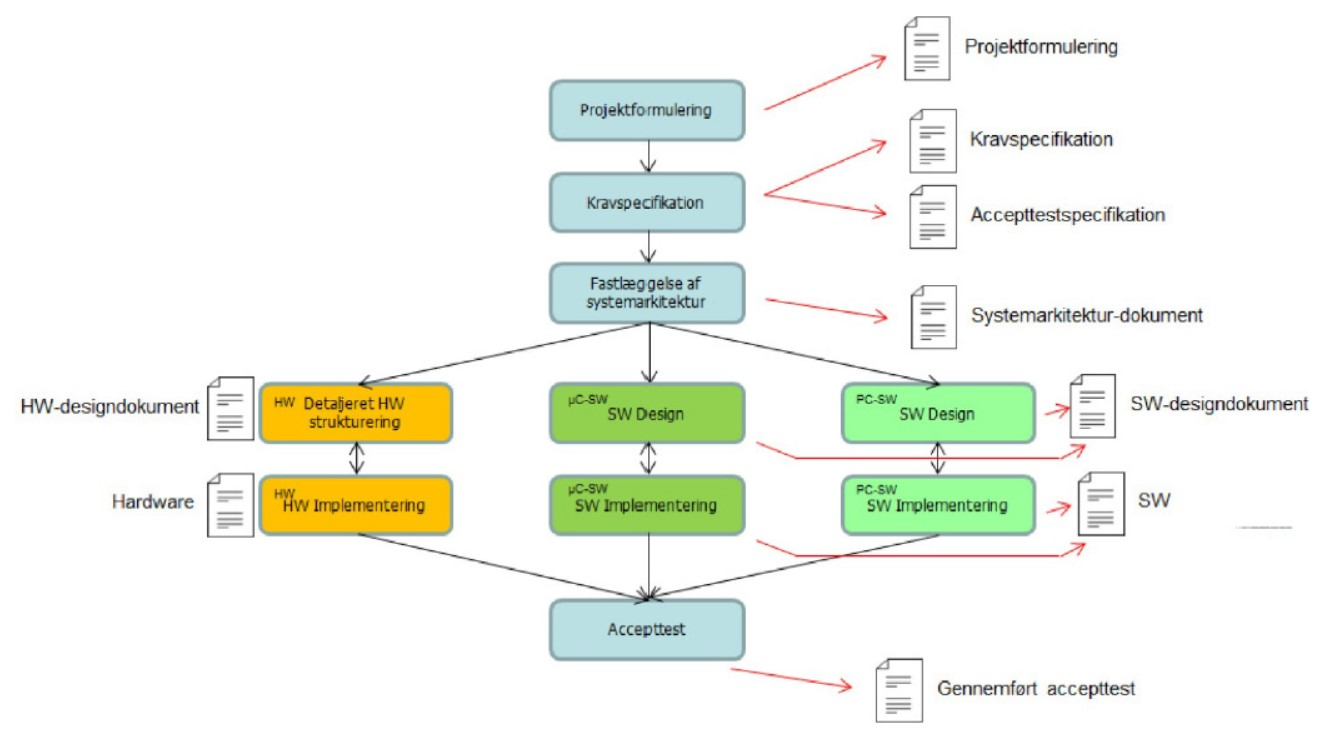
\includegraphics[width =1.0\textwidth , center]{billeder/ASEmodellen}
\caption{ASE-modellen.}
\end{figure} 
Kravspecifikationen bliver specificeret som en række Use cases ud fra problemformuleringen. Use cases benyttes til at beskrive aktørernes interaktion med systemet. Sammen med de ikke-funktionelle krav opnås der med Use casene et overblik over hvilke krav der stilles til systemets funktionalitet. Systemets design bestemmes igennem hardware og software design og implementering, herefter kan en accepttest udarbejdes. Ved udførelsen af accepttesten tjekkes det at kravene er opnået.
\subsection{V-modellen}
V-modellen en model som er faseopdelt udviklingsmodel. Denne model beskriver udviklingsfaserne og testfaserne i et projekt sideløbende. V-modellem er blevet benyttet sideløbende med ASE-modellen. Specifikationen af test foregår parallelt med udviklingen af selve systemet i V-modellen. Fordelen ved denne model er at testene sker på forskellige niveauer, hvilket sikre at udviklede delsystemer virker som ønsket. Det vigtige her er at en fase er færdiggjort, inden den næste fase påbegyndes. 
\begin{figure}[H]
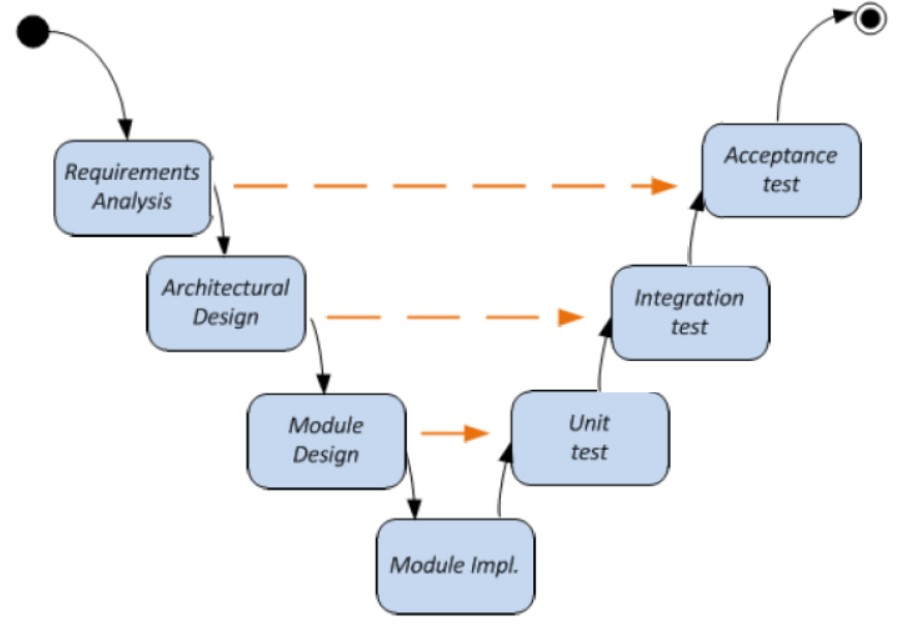
\includegraphics[width =0.7\textwidth , center]{billeder/Vmodel}
\caption{V-modellen.}
\end{figure} 
Ud fra modellen ses det at den første fase er udviklingen af kravspecifikationen. Her udarbejdes der en tilhørende accepttest, denne test gør det muligt at tjekke om systemet til sidst lever op til de opstillede krav. Den næste fase er herefter systemarkitektur, her udvikles den tilhørende test, denne test undersøger integrationen mellem de implementerede moduler. De sidste to fase af udviklingsfasen er design og implementering af systemets enkelte moduler, her udføres enhedstesten løbende af de implementerede moduler.
\subsection{Vandfaldsmodellen}
Vandfaldsmodellen er en model der bruges til udvikling af software, hvor softwareudviklingen betragtes som værende konstant løbende nedad. Her kan udviklingen af et modul i en ny fase først påbegyndes når den foranliggende fase er afsluttet. Denne model et i projektet benyttet til udviklingen af softwarearkitekturen. 
\begin{figure}[H]
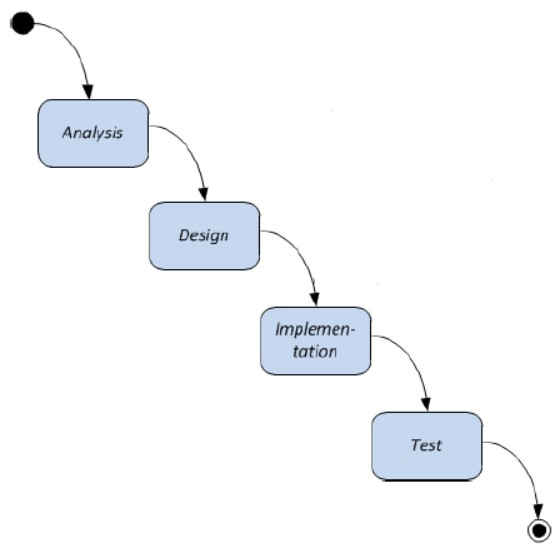
\includegraphics[width =0.5\textwidth , center]{billeder/Vandfald}
\caption{Vandfalds modellen.}
\end{figure} 
Disse tre modeller; ASE-modellen, V-modellen og vandfalds-modellen arbejder alle i en kronologisk logisk rækkefølge. Modellerne er benyttet i et omfang, hvor de har kunnet supplere hinanden. ASE-modellen giver det store overblik, mens V-modellen sikre udarbejdelsen af de nødvendige tests. Vandfalds-modellen er den proces, hvilken der er arbejdet ud fra i alle projektets facetter.   
\subsection{Projektstyring}
Ledelsen
Tidsplan
Opdeling
Github
SCRUM
- Pivoval tracker
\section{Metode}
UML
SysML
- Beskrivelse af modellerne
	- BDD
	- IBD
	- Domæne
	- Sekvens
	- Applikation
	- Klasse diagrammer
	- Software (black box?)
	
	
	
	\section{Specifikation og analyse}
	??
	Beregninger til hardware
	\section{Arkitektur}
	\subsection{Hardware design}
	kort indledning
	Hardware beskrivelse
	Signalets vej
	BBD indsættes
	\subsection{Software design}
	Kort indledning
	\section{Design, implementering og test}
	PUSH
	Observer/subject
	QUEUE
	
	
	
	
\section{Resultater og diskussion}
Hvad er der kommet frem til
\section{Udviklingsværktøjer}
Til udviklingen af produktet, og dermed igennem hele projektarbejdet, er der blevet brugt en række udviklingsværktøjer. Følgende er disse udviklingsværktøjer beskrevet yderligere.
\subsection{Microsoft Visio 2010}
Tegneværktøjet Microsoft Visio, er blevet anvendt i forbindelse med design af både UML og SysML diagrammer. Microsoft Visio er det oplagte valg til at designe disse diagrammer, da programmet søger for at diagrammerne får et enkelt udseende og tydeligt kommunikerer til læseren, hvad diagrammerne vil vise.
\subsection{Visual Studio 2013}
Programmeringskoden til projektet er blevet skrevet i C\#. Her er Visual Studio 2013 blevet anvendt som kompiler. Dette program er blevet valgt da Visual Studio gør det nemt at omskrive ideer og tekst til kode, som derefter kan omskrives til metoder. Desuden indeholder Visual Studio 2013 funktionen Windows Form Application. Denne funktion gør at de ønskede resultater fra programmets metoder visuelt kan fremstilles.
\subsection{NI Multisim 13.0 med Ultiboard 13.0}

\subsection{NI-DAQmx}
NI-DAQmx, også omtalt NI-DAQ, er et værktøj som er blevet udarbejdet af National Instrument. Dette værktøj anvendes til at forstærke det indkommende signal. Dette signal kommer fra hardwaren. NI-DAQ omdanner desuden signalet fra et digitalt signal til at være et signal der kan bruges i kode øjemed. 
\subsection{Analog Discovery fra Digilent and Analog Devices}
Analog Discovery er i projektet den der benyttes om en waveform-generator. Det er derfor Analog Discovery der benyttes til at teste systemet. Dette sker ved at der sendes et sinus signal ind i systemet, som systemet derefter skal behandle.
\section{Opnåede erfaringer}
Hvad er erfaret
 - hardware
 	- forskellige måder at lave det samme på.
 - programmering
 	- oberserver subject
 	- Push
 	- tråde
reviews
\section{Fremtidigt arbejde}
Iltmætning
Få produktet til at virke på en patient
Andet fremtidigt
Både indenfor hardware og software
\chapter{Konklusion}
Afrunding
konkludering
Hvad lykkedes og hvad lykkedes ikke
\chapter{Referencer}